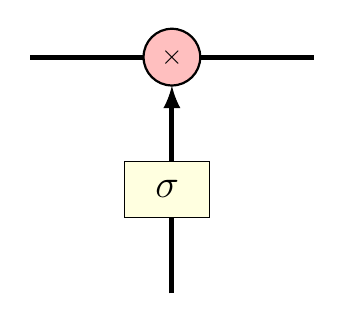
\begin{tikzpicture}[scale=2.4]

% The grid
% \draw[step=0.5, gray!40, very thin] (0,0) grid (8,4);

% LSTM frame
\def \yONE {1.5}
\def \yTWO {4.3}
\def \sigmoidWidth  {0.45}
\def \sigmoidInDist {0.2}
\def \sigmoidHeight  {0.3}
\def \yB  {2.3}
\def \yD  {3.75}
\def \shift {0.3}
% First Sigmoid
\draw[fill=LightYellow] (2, \yB+.6) rectangle (2+ \sigmoidWidth, \yB +.6+ \sigmoidHeight) node[pos=0.5] {\Large$\sigma$};

\def \r {.15cm}
% The Upper times operator % first time from left
\draw[thick, fill=pink] (2.25, \yD) circle (\r) node {$\times$};

\draw[line width=1.8pt]  (1.5, \yD) -- (2.1, \yD);
\draw[line width=1.8pt]  (2.4, \yD) -- (3, \yD);


%%%%first line from left from sigmoid ft till times input from C_{t-1}
\draw[line width=1.8pt]  (2.25, \yB +.2) -- (2.25, \yB+.3 +\sigmoidHeight);
\draw[arrows=-latex, line width=1.8pt]  (2.25, \yB+.3 +\sigmoidHeight+\sigmoidHeight)--(2.25, \yD-.15);

\end{tikzpicture}